


\begin{figure}[H]
\centering
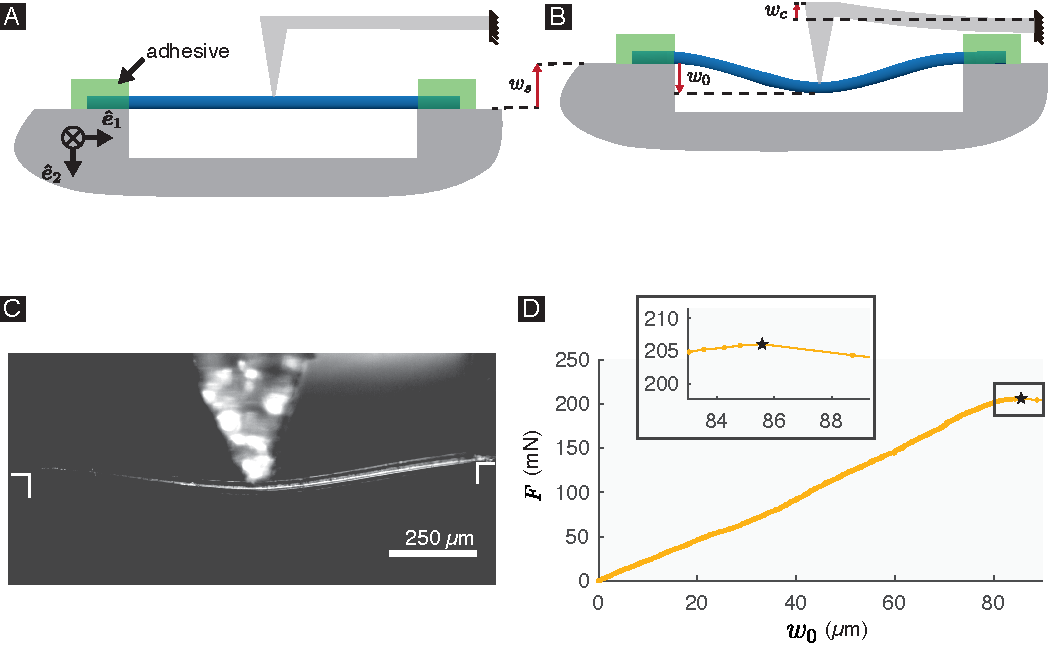
\includegraphics[width=\textwidth]{Figures/FixedFixed_V3.pdf}
\caption{
Description of three-point bending test setups and data obtained from the tests.
(\textsf{A}) and (\textsf{B}) are schematics of the fixed-fixed test setup of a spicule. In contrast with the simply-supported test setup, adhesive is applied over the spicule's ends to prevent it from sliding or rotating during the test.
Schematics (\textsf{A}) shows the reference configurations, while schematics (\textsf{B}) shows the deformed configurations. The mid span specimen displacement, $w_0$, cantilever deflection, $w_c$, and stage displacement, $w_s$, are marked in (\textsf{A}) and (\textsf{B}).
Basis vectors $\physe_1$ and $\physe_2$ are shown in (\textsf{A}). Basis vector $\ethree$ points into the plane of the paper.
}
\label{fig:FFconfig}
\end{figure}
